%% This is an example first chapter.  You should put chapter/appendix that you
%% write into a separate file, and add a line \include{yourfilename} to
%% main.tex, where `yourfilename.tex' is the name of the chapter/appendix file.
%% You can process specific files by typing their names in at the 
%% \files=
%% prompt when you run the file main.tex through LaTeX.
\section{Introduction}

Paper airplanes are more than children's toys; they foster creativity and inspire elegant engineering solutions in all generations. 
Due to the simplicity in construction, thousands of paper airplane designs have been explored. For example, the Guinnes World Record 
paper airplane, "The Glider",  was capable of staying in air for an astounishing $15.4$s.  

These designs differ widely in paper material, wing geometry, 
and body shape; nevertheless, they are all governed by the same aerodynamic principles. This paper aims to investigate these principles
 on a theoretical as well as an empirical basis. More specifically, we focus on two topics: flight stability and lift vs drag relation. 
Theories are first discussed, and then experiments are performed to illustrate the principles. Due to our limited access to scientific 
equipment, most of the experiments performed are crude in nature and should be examined qualitively instead of quantitatively. We discovered
that our experimental results are consistent with previous researches and demonstrate the validity of existing aerodynamical theories.

\begin{figure}[hl]
	\centering
		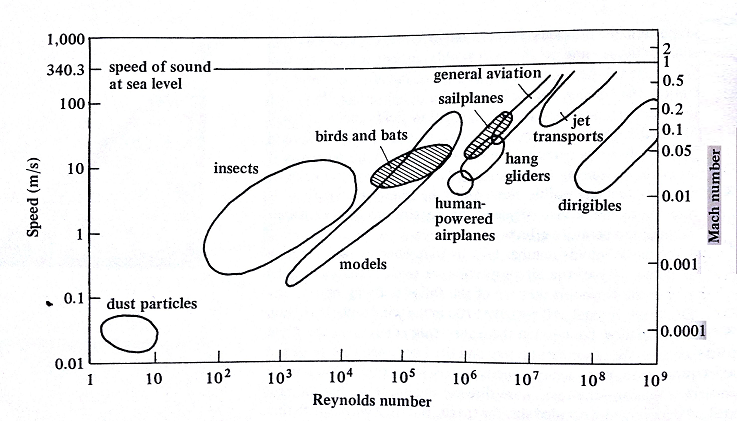
\includegraphics[scale=.5]{figures/reynoldsrange.png}
		\caption{Reynolds-number range of a variety of aerodynamic objects in nature and technology. Reynolds numbers are given as a function of Mach number and speed. The ranges indicated for the different types of flying objects are approximate. Figure adapted from \cite{wegener}}
	\label{fig:reynoldsrange}
\end{figure}


Paper airplanes have similar Reynolds-number range as insects (see Figure~\ref{fig:reynoldsrange}). Furthermore, they have similar weight and wing thickness as
insects. As a result, the findings from this paper may be applied to the widely studied fields of insect aerodynamics. The complex fight mechanism of insects may
be modeled using an appropriately folded paper airplanes.
